% !TeX spellcheck = en_US

Das ist die Methode.

\section{Phospholipids}
\label{section:metodeLipide}

Phospholipids are the building block of membranes in nature. They own two long hydrophobic chains and a polar head. A membrane is a bilayer of Phospholipids with the hydrophobic parts showing inwards and the hydrophilic head pointing outwards. They are also natural detergents, as they can bind to hydrophobic waste and forming an emulsion, making them removable with polar liquids like water \cite{SriramaM.BhairiPh.D..}.

Phospholipids are generally solvable in Alcohols(???). To apply Phospholipids, the solution is given on the surface. When the solvent dries out, the lipids are bining to the surface creating a layer. this layer can be solved again with the same solvents. If the ice layer is held by lipids, they can be used as a sacrificial layer, being solved at cryogenic temperatures. But to solve this layer, a high solubility at cryogenic temperatures must be given as the surface of the sacrifical layer is only on the edge of the sample.

\subsection{Parylene}

One idea of balancing Hydrophilic and Hydrophobic characteristics is to use Parylene. Parylene is superhydrophobic (SOURCE??? MAYBE NOT), which helps ice not to adhere to the surface. But used alone, an ice layer could not be frozen on top with plung-freesing or by hand as a water drop would not spread on the surface. 

For this reason, lipids are used in combination with parylene. The lipids are holding the Ice layer onto the parylene. With a solvent, the lipids can be solved and the parylene will prevent the ice layer to hold on the slide, detaching the layer. Or mechanical pulling on the ice is easier, as parylene is preventing not perfectly covered pieces from adhering on the slide.

\subsection{Preparation lipids and cover glass}

To create the slides with parylene and lipids, cover glasses (5 mm diameter) is first coated with a thin layer of parylene. Then the slides are dipped into lipid solution, covering the whole surface in lipids. then the slides are dried, so lipids can settle on the surface. 

Two different lipids are used: DOPC and EGG-PC. DOPC is storaged in powder form. The first step is to solve the DOPC Powder in Ethanol (25 mg / 1 ml). Then, the solution is transferred into several small bottles. EGG-PC is shipped solved in chloroform. Two different ratios were used: 25mg / 1 ml and 10 mg / 1ml. the phioles were broken and then also transferred into several small bottles. small bottles were chosen because if solution is coating the threads of the cap, the bottle cannot be closed airtight anymore, leading to evaporation in the flask. By splitting it into multiple flask and using the solution, only one bottle with a small part of the solution is not airtight.

\subsection{solubility lipids}

Two different solubility experiments are proposed. The first is at room temperature to find solvents which work generally at higher temperatures. With the results, first solution which don't solve the lipids can be left out of the next experiment, as there are only limited baths available. The next one is at cryogenic temperatures to find solvents which also work at cryogenic temperatures.

These tests are conducted to find a fluid to solve a sacrificial layer out of lipids.

\begin{figure}[hbt!]
	\centering
	\begin{picture}(6,3)
		 \multiput(0,0)(6,0){2}{\line(0,1){1.25}}
		 \put(0,0){\line(1,0){6}}
		 \multiput(0,.5)(0,.25){4}{\line(1,0){6}}
		 \multiput(0,0)(0.5,0){12}{\line(1,1){0.5}}
		 \multiput(6,0.5)(-0.25,0){24}{\line(-1,1){0.25}}
		 %beschriftung
		 \thicklines
		 \put(-1,.25){\vector(1,0){1}}
		 \put(-1,.25){\makebox(0,0)[r]{Slide}}
		 \put(7,.625){\vector(-1,0){1}}
		 \put(7,.625){\makebox(0,0)[l]{Parylene}}
		 \put(-1,.875){\vector(1,0){1}}
		 \put(-1,.875){\makebox(0,0)[r]{Lipid Layer}}
		 \put(7,1.125){\vector(-1,0){1}}
		 \put(7,1.125){\makebox(0,0)[l]{Ice}}
	\end{picture}
	\caption{Sacrificial layer}
	\label{fig:sacrificial layer}
\end{figure}

\subsubsection{at room temperature}

First, the potential solvents are picked. For that, the tested liquids needs to be save for humans in such way that no extractor hood is needed. This is needed because the following experiment does not fit under an extractor hood. The tested substances are 4-Methyl Pentene, 3-Methyl Pentene, 1-Pentene, Isopentane, 1-Propanol, Pentane and Ethanol. Each liquid is put in a separate bottle. Then the slides are prepared  as previously described.

Then a slide is placed inside each potential solvent. After 15 minutes, the slides are removed and examined under a microscope. then the results are documented in a list. Solvent which managed to solve all lipids off the slide are now tested at cryogenic temperatures.

\subsubsection{at cryogenic temperature}
\label{chapter:meltingtemp}

As solubility is very temperature dependent, a test is conducted at -140°C. The general process is the same, but the liquids are given in liquid nitrogen cooled baths, which are regulated to the desired temperature. 

The Freezing point of tested Solutions are not all below -140°C (Table \ref{table:SchmelztemperaturLösungsmittel}).
To still test the solubility, they are partially tested at temperatures slightly above their freezing point. Also solution with a high freezing point are mixed with solution with a low freezing point as an attempt to reduce their freezing point.

\begin{table}[hbt!]
	\centering
	\begin{tabular}{|l|c|}
		\hline
		solvent & melting point in °C \\
		\hline
		\hline
		4-Methyl Pentene & -154 \\ 
		\hline
		3-Methyl Pentene & -154 \\
		\hline
		1-Pentene & -165 \\
		\hline
		Isopentane & -160 \\
		\hline
		1-Propanol & -126 \\
		\hline
		Pentane & -129 \\
		\hline
		Ethanol & -114 \\
		\hline
	\end{tabular}
	\caption{Melting Point in °C for tested solvents.}
	\label{table:SchmelztemperaturLösungsmittel}
\end{table}

In the end, the experiment has proven that solving lipids fast and reliable is not possible with tested solvents. As all solvent lipid combinations seem to be endothermic, finding a working solvent lipid combination is very unlikely.

Additionally, some solvents tested are soluble in water. It is unknown whether the solvents could be solved or diffuse inside the ice layer at -140\,°C. Therefore the ice layer could be changed in some undesired manner. if a final solvent is found which is soluble in water, this needs to be addressed an tested in future experiments.

\section{"finger"}

The next tested method is detaching the ice layer mechanically. For this, a lifting assembly is used. To make this possible, the bottom layer is varied to reduce the adhesion of the ice. Also, as the assembly was not used in similar work before, different variables are addressed and examined.  

\subsection{Assemblies used at cryogenic temperatures}

The assembly used to lift up samples is called finger. The finger has two main parts: A metal rod with a slightly pointed tip (Fig. \ref{fig:querschnittfinger}). Near the tip, the rod is also temperature controlled with a temperature sensor and a heater. On the tip, a glue like HFE can be used to glue onto the sample. The second main part is a 3D printed part, containing the outer shell and routing of the cold gaseous nitrogen. The nitrogen is first flowing inside and around the metal bar for cooling. then, the Gas is flowing through an outer mantle for additional cooling and out on top.

The finger is  mounted on three stages and a track. the three stages allow fine adjustment of the finger position in X,Y and Z axis. Also, when the finger is sticking to a surface, force can be applied by moving the stages in either direction. The Finger can also be moved along the rail. In use, the assembly is clamped down on the rail, to prevent additional movement. when not in use, the assembly can be moved on the rail further back. this allows access beneath the finger.

\begin{figure}[hbt!]
	\centering
	\begin{overpic}[height=7cm]{TempFinger}%
		%\color{red}%
		%\put(49,48){\vector(0,-1){10}}%
		%\put(49,48){\makebox(0,0)[cb]{Mitte}}%
		%Beschriftung:
		\thicklines
		\put(42,15){\vector(-1,0){10}}
		\put(42,15){\makebox(0,0)[lb]{ Heater,}}
		\put(42,15){\makebox(0,0)[lt]{ Temperature sensor}}
		\put(3,50){\vector(1,0){20}}
		\put(3,50){\makebox(0,0)[r]{Steel Rod }}
		\put(5,96){\vector(1,-1){10}}
		\put(5,96){\makebox(0,0)[r]{Gas inlet }}
		\put(48,96){\vector(-1,-1){10}}
		\put(48,96){\makebox(0,0)[l]{ Gas outlet}}
		\put(17,0){\vector(2,1){10}}
		\put(17,0){\makebox(0,0)[r]{Tip }}
		% Gas Flow:
		%\put(21,45){\vector(0,-1){12}}
		%\put(19,33){\oval(4,4)[b]}
		%\put(17,33){\line(0,1){12}}
	\end{overpic}
	\caption{Querschnitt finger}
	\label{fig:querschnittfinger}
\end{figure}


HFE (LANGES WORT) is an oil typically used as an cryoimmersion fluid \cite{Faoro.2018b}QUELLE ÜBERPRÜFEN!. Besides that, it has temperature dependent abilities. At freezing temperatures, it does not freeze into a solid at once. It gets more and more viscious before it freezes completely. this temperature dependency is used to first apply the HFE at higher temperatures with low viscosity and pull on the sample at low temperatures.

There are two ways of transporting samples around the work station. The shuttle fits inside the harbor. one sample can be fixed on it with screws and a brace with a hole called "window". The hole in the window exposes the upper side of the sample, allowing access for the finger and microscopy. On the other hand, small container with space for three $\varnothing$\SI{5}{\milli\meter} samples are used. These are 3D Printed, modified version of other containers, which can be stored in Sets of 12 in a long term storage.

FIGURE CONTAINER AND SHUTTLE.

In the beginning a smaller bath is used (Fig. \ref{fig:KleinesBad}). The Small bath contains two floors. The second floor is exposed and used for work. embedded in the floor are container holder, allowing transport and storage of samples. Then three elevated baths are installed for other Liquids or tools. Also a Haven for a shuttle is installed which is used for the microscopy. The small baths and the haven is elevated over the second floor, so a temperatures over \SI{-195.8}{\degreeCelsius} can be regulated. The whole assembly is insulated by Nitrogen gas flowing inside the wall of the bath. Then the Nitrogen gas is blown from the brim radially to the rotation axis. The nitrogen gas separates the damp air in the room with the dry nitrogen gas inside the bath, preventing ice to form inside the bath.

This small bath can also be used with a finger. But this has some limitation: first, the space is small. The finger can be moved, but the space limits work with pincers. Additionally, the smaller baths are not needed for using the finger. also the Shuttle needs to be tilted in a specific angle so the shuttle can be moved in and out of the haven. The work flow also allows only one Shuttle in use at once, limiting throughput. Also Liquid nitrogen needs to be refilled quickly.

\begin{figure}[hbt!]
	\centering
	\begin{overpic}[width=10cm]{SmallBath}
		\put(40,25){\vector(1,1){10}}
		\put(40,25){\makebox(0,0)[r]{Shuttle Haven}}
		\put(25,45){\vector(1,0){10}}
		\put(25,45){\makebox(0,0)[r]{Tool Bath}}
		\put(73,35){\vector(-1,1){10}}
		\put(73,35){\makebox(0,0)[l]{Ethanol Bath}}
		\put(73,27){\vector(-1,1){10}}
		\put(73,27){\makebox(0,0)[l]{HFE Bath}}
		\put(49,76){\vector(-0.15,-1){3.4}}
		\put(51,76){\vector(0.15,-1){3.4}}
		\put(50,76){\makebox(0,0)[b]{container holder}}
		\put(75,78){\vector(-2,-1){10}}
		\put(76,78){\vector(-1,-2){4.5}}
		\put(75,78){\makebox(0,0)[b]{outlets}}
		\put(75,80){\makebox(0,0)[b]{Nitrogen Gas}}
		
	\end{overpic}
	\caption{Small Bath.}
	\label{fig:KleinesBad}
\end{figure}

During this master thesis, a second bigger bath is build (Fig. \ref{fig:GroßesBadMitFinger}). In general, the structure is similar. It also has a second elevated floor which is fabricated out of two plates screwed together. it also has indents for containers. No baths are installed, but space is held free for later addition of small baths. Also two harbors can be mounted for parellel work on two shuttles. Also both harbors can be mounted either flat or with an angle. The Bath is insulated with styrofoam and a rim with holes for warm nitrogen gas is placed on top. The holes are places along the inside of the longer side, so the stream covers the whole area with minimal turbulence. This also keeps the inside ice free.

\begin{figure}[hbt!]
	\centering
	\begin{overpic}[width=7cm,grid]{BigBathWithFinger}
		
	\end{overpic}
	\caption{Big Bath with Finger.}
	\label{fig:GroßesBadMitFinger}
\end{figure}

The Shuttles are also used in cryo light microscopes. The Microscope used for cryotemperatures have an additional box installed, routing Cold nitrogen gas underneath a harbor, where the sample is placed. Heaters are placed around the box and under the harbor to archieve a constant temperature. On top of the Harbor, warm Nitrogen is blown so no ice is forming inside the optical path.

\FloatBarrier

\subsection{general process}

The goal is to mechanically lift a piece or the whole ice layer off the slide it is frozen to. The challenge is that the sample needs to stay at a vitrified state. The "finger" as previously explained is a device which can lift at a temperature range which guarantees that the sample stays vitrificated. 

The process has following steps: First, if not already done, cool down the finger to -140\,°C. The sample is prepared and fixed onto a shuttle in the harbor underneath  the finger.Then, HFE is applied on the tip. Then, the finger is positioned with the stages over the sample. After checking from different sides an camera, the finger is lowered onto the sample. Then the temperature is reduced and waited until the sample and finger is cooled down. Then the finger is pulled up by turning the stage until it detaches from the sample. After this step, if detaching was successful, the shuttle is changed to an empty shuttle. the Piece is lowered onto it and the piece is unglued by lowering the temperature. then the piece is fixed onto the shuttle.

To collect first insight, samples with parylene and lipids (as described in Section \ref{section:metodeLipide}) are used. by doing those experiments, different variables where determined which could significantly influence of successful detaching. Then the different variables are examined with different experiments to improve the finger. Following variables are determined: the amount of HFE can affect the maximum force and can be falsely applied, the temperature also affects the maximum force, tensile forces and shear forces, the thickness of the ice layer, the layer between slide and ice. In the following, I will examine those in greater detail.

\subsection{determining needed amount of glue}

Using the correct amount of HFE as glue is important for a high repeatability. Too little glue is not able to connect the finger to the sample. too much glue results into a thicker layer, which is the weakest link between finger and sample. additionally, the glue can spread underneath the "window" which is holding down the sample onto the shuttle. 

In first experiments, the HFE used as glue was applied with a pincer. TO archieve this, the HFE is given in a cold bath at -140°C. This stops HFE from evaporating. The thickened hfe is now scooped with pincers on the tip of the finger. Though the correct amount is only determinable qualitative.

As an effort to determine the correct amount of HFE a pipette is used. The HFE is pipetted at room temperature, because at lower temperatures the viscosity is already too high. While applying the HFE onto the desired surface, around $4\,\mu l$ is already evaporating. Also, sometimes the hfe does not land on the tip but on the side of the tip, where it is not very useful. 

In the first experiment, I dosaged three different amount onto the tip of the finger with the pipette. The amount on the finger did not correspond to the amount of HFE. So other variablilities like the time between loading and unloading and hitting the correct spot on the finger is more relevant than the amount of HFE used.

To still determine the correct glue amount, two pictures representing the lowest and the highest usable HFE amount was picked. then the volume is calculated. this can be used as reference for future work for dosaging the right amount of HFE.

\subsection{temperature test}

Ethoxynonafluorobutane, also called HFE 7200, has a melting point of \SI{-138}{\degreeCelsius}. Below, HFE gets increasingly viscious until it is hard and brittle. This property can be used as a temperature controlled glue. 

In use three mode with different temperatures exist: first in "unglue" node, the shuttle and the finger is held at \SI{-140}{\degreeCelsius}. HFE has a low viscosity, which allows application on the sample. Also detachment without breaking the sample is possible. in "glue" the shuttle and the finger are cooled to \SI{-160}{\degreeCelsius}, HFE hardens and force can be applied to detach the ice layer. then, "thaw" cleans the finger by heating the tip to \SI{20}{\degreeCelsius}. 

As HFE is getting harder with temperature, lower temperatures in the "glue" state could allow higher forces to reliably detach the ice layer. To test this hypothesis, HFE is examined at temperatures until \SI{-170}{\degreeCelsius}. (DESCRIPTON??? VIELLEICHT?)

\subsection{tensile- vs shear mode}

The direction of force is also a factor which can easen liftoff of ice. Tensile mode an shear mode can be currently applied with the finger. Tensile modes advantage is the easy application with the finger. But for separating layers, this mode takes more force, as a bigger area adhering on the slide take the forces of the finger. The tensile mode would take less force, but removing a smaller part off the surface is difficult.

In application, the shuttle is tilted around 15 degrees for easier access to the shuttle. The finger is also tilted so the tip is parallel to the shuttle. To apply force, the finger can be pulled by stages in either X, Y, or Z direction. For each direction, the stress can be split into tensile and shear stress. In Z direction, mostly tensile stress is applied (Fig. \ref{fig:tensilevsshear} (a)). in X direction, mostly shear stress is applied (Fig. \ref{fig:tensilevsshear} (b)). In Y direction, only shear stress is applied, but will result in shattering of the sample, as the Ice layer is clamped down which will not allow sideways motion.

\begin{figure}[hbt!]
	\centering
	\input{../images/Zeichnung_finger_Tensile_vs_Shear.pdf_tex}
	\caption{Tensile vs Shear mode}
	\label{fig:tensilevsshear}
\end{figure}

\subsection{ice thickness and vitrified ice}

To lift off a piece of ice from the ice layer, the layer must be broken in some way. Also, thicker ice sheets are harder to break than thinner ice sheets, simply of the cross section of the layer. Again, the extend of this factor is not forseeable. 

Initially, to save time for experiments, the samples are freezed by Hand in liquid nitrogen, as described before. However, the ice layers are less consistent compared to plunge freezing, resulting in mostly thicker ice layers compared to plunge freezing. also as the sample is frozen in liquid nitrogen, the leidenfrost effect is inhibiting the formation of vitrified ice. 

To compare the influence of hand freezing and plunge freezing, results of lifting off samples frozen with both methods are compared. No other factors are varied in those experiments. In the end, hand freezing and plunge freezing did not make a difference. Therefore, hand freezing was also applied in future experiments, as this effect is determined as neglegtable compared to other factors.

\section{PDMS}

PDMS is as stated before a coating which is used for passive deicing. It is hydrophobic and has a low surface energy. Also it can be coat spinned into a thin layer, which is needed in this application. Also it is widely available and tunable. The only downside is that the surface needs to by hydrophile when plunge freezing. The simplest method is using a Plasma generator.

Plasma curing is also used for PDMS in Bonding (QUELLE). Also PDMS can reach under certain condition a glass like state, which makes the surface brittle and reduces the adhesion forces further (PAPER). This was done by mixture ratios of 50:1 to 100:1. Also, Plasmacuring makes the surface temporarily hydrophilic by polarizing the surface. But this is destroyed by contact of any material. Still, plasma treatment is influencing the adhesion of the ice, making it harder to remove.


Additionally,as PDMS is hydrophobic, plasmatreatment is used to make the surface more hydrophilic. Additionally, plasma treatment is changing the structure of the PDMS. 

I found that plasma treatment has different effects on the PDMS on different mixture ratios. 

\subsection{Preparation of PDMS samples}

I used Dowsil Sylgard 184 Silicone elastomer as PDMS \cite{DOW.}. It has two component, Base coat and curing agent. Depending on the Mixture ratio of these two components, the PDMS gets different properties. 

All PDMS samples are prepared in a similar way only warying minimal in a couple of steps. The preparation starts with weighting out the needed amount of base coat and curing agent. The mixture is then stirred intensively. The mixture is placed under a vacuum bell to gas out air bubbles. Meanwhile the slides are cleaned with ethanol or isopropanol and dried. Afterwards, the PDMS mixture is coat-spinned on the slides. Then the coated cover glasses are baked in the oven.

For 1:2 base coat to curing agent weight ratio, the PDMS mixture is comparably liquid. A vacuum of \SI{30}{\min} is used. A coat spinning time of \SI{120}{\minute} at \SI{3000}{\rpm} is results in a smooth surface for all used slides. The baking time should be at least \SI{24}{\hour} by \SI{80}{\degreeCelsius}. For shorter baking times, plasma treatment has a slighlty different effect. Normally, touching a treated area will neutralize the effect of plasma treatment like hydrophility only locally on the touched surface. But here, touching the surface leads to the complete neutralization of plasma treatment when touching. In this work, the effect is undesired. 
 
For 4:1 base coat to curing agent weight ratio, the PDMS is more viscious. The Vacuum and coat spinning are the same for \SI{30}{\min} vacuum and \SI{3000}{\rpm} for \SI{120}{\minute}. But a baking time of \SI{30}{\min} at \SI{80}{\degreeCelsius} is already sufficient to harden the PDMS. 

For 50:1 base coat to curing agent weight ratio, the PDMS mixture is as viscious as the base coat. A longer vacuum of \SI{1}{\hour} is needed to air out all bubbles. Because of the higher viscosity, the coat spinning is increased to \SI{3500}{\rpm} for \SI{180}{\minute} (NACHSCHAUEN). Also a longer baking time of \SI{20}{\hour} at \SI{80}{\degreeCelsius} is needed to harden the PDMS. 

Additionally, rectangular cover glass with 20x20 and 40x20 (NACHSCHAUEN) are coat spinned and split in multiple smaller pieces to speed up the sample preparation process. The process is the same described as before for each PDMS mixture ratio, but with two additional steps.

Before coat spinning, the glass is scratched with a diamont Pencil (?)
Glas vorher anritzen

Glas teilen in kleinere teile


\subsection{Influence of plasma treatment on PDMS}

\subsubsection{setup}

To test the tensile strength of different PDMS mixtures and the effect of plasmacuring, a Pulling machine (NAME RAUSFINDEN)is used. 
On the Top part, two sensors are installed. The upper Sensor is rated for \SI{2}{\kilo\newton}(ÜBERPRÜFEN). the lower sensor is rated for up to \SI{100}{\newton}. As the upper one is extremely stiff and the forces are \SI{<<2}{\kilo\newton}, the upper Sensor can be assumed as inflexible. On both the upper and lower part, two clamps are fixed onto the machine. On the Bottom Clamp a 3D-Printed stage is used with threaded holes for screws. 

Glass slides with coated PDMS are used, which are fixed on the bottom end of the machine (Fig. \ref{fig:PullingMachineSetup}). On the top end, waterjet cut stams are clamped on. Then a drop of uv glue is put on the top part. the top part is lowered onto the bottom side. Then the uv glue is cured with an uv pistol for 3 minutes (1.5 minutes from the left 1.5 minutes from the right). Then the the sample is pulled with constant distance.

\begin{figure}[hbt!]
	\centering
	\begin{subfigure}[]{0.45\textwidth}
		\centering
		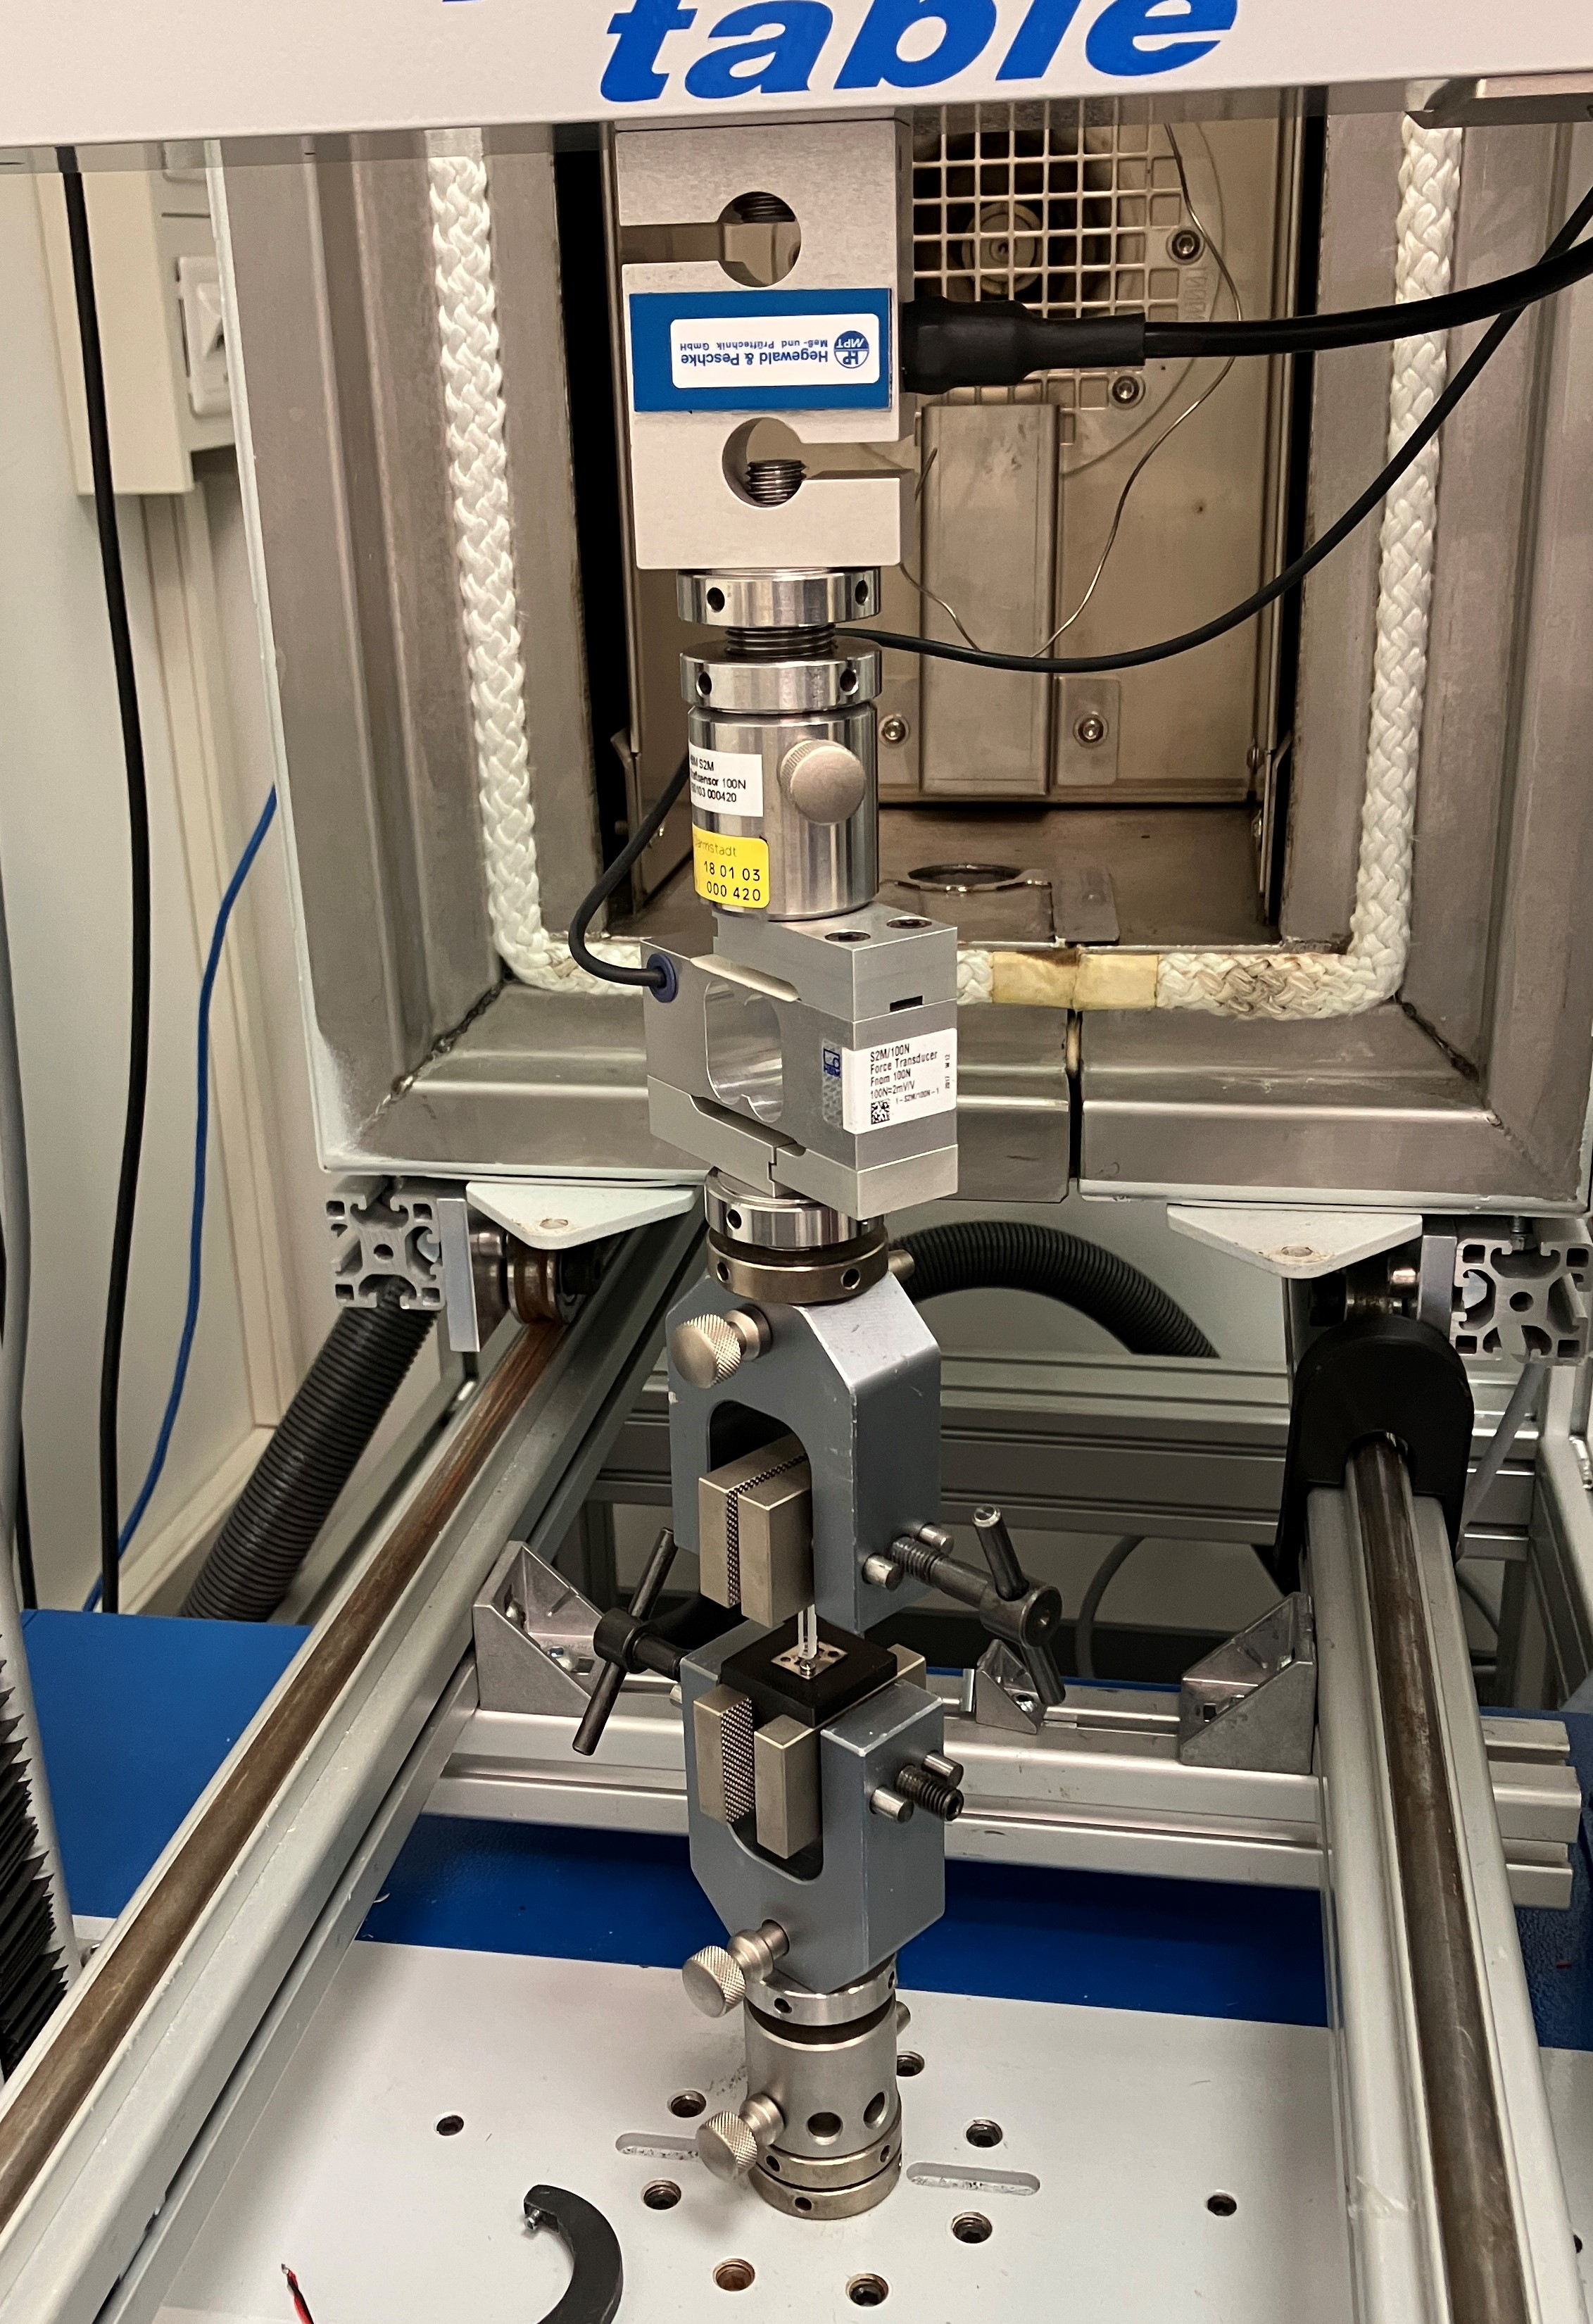
\includegraphics[width=6cm, height=9cm]{AufbauPullingMachine}
		\caption{}
	\end{subfigure}
	\begin{subfigure}[]{0.45\textwidth}
		\centering
		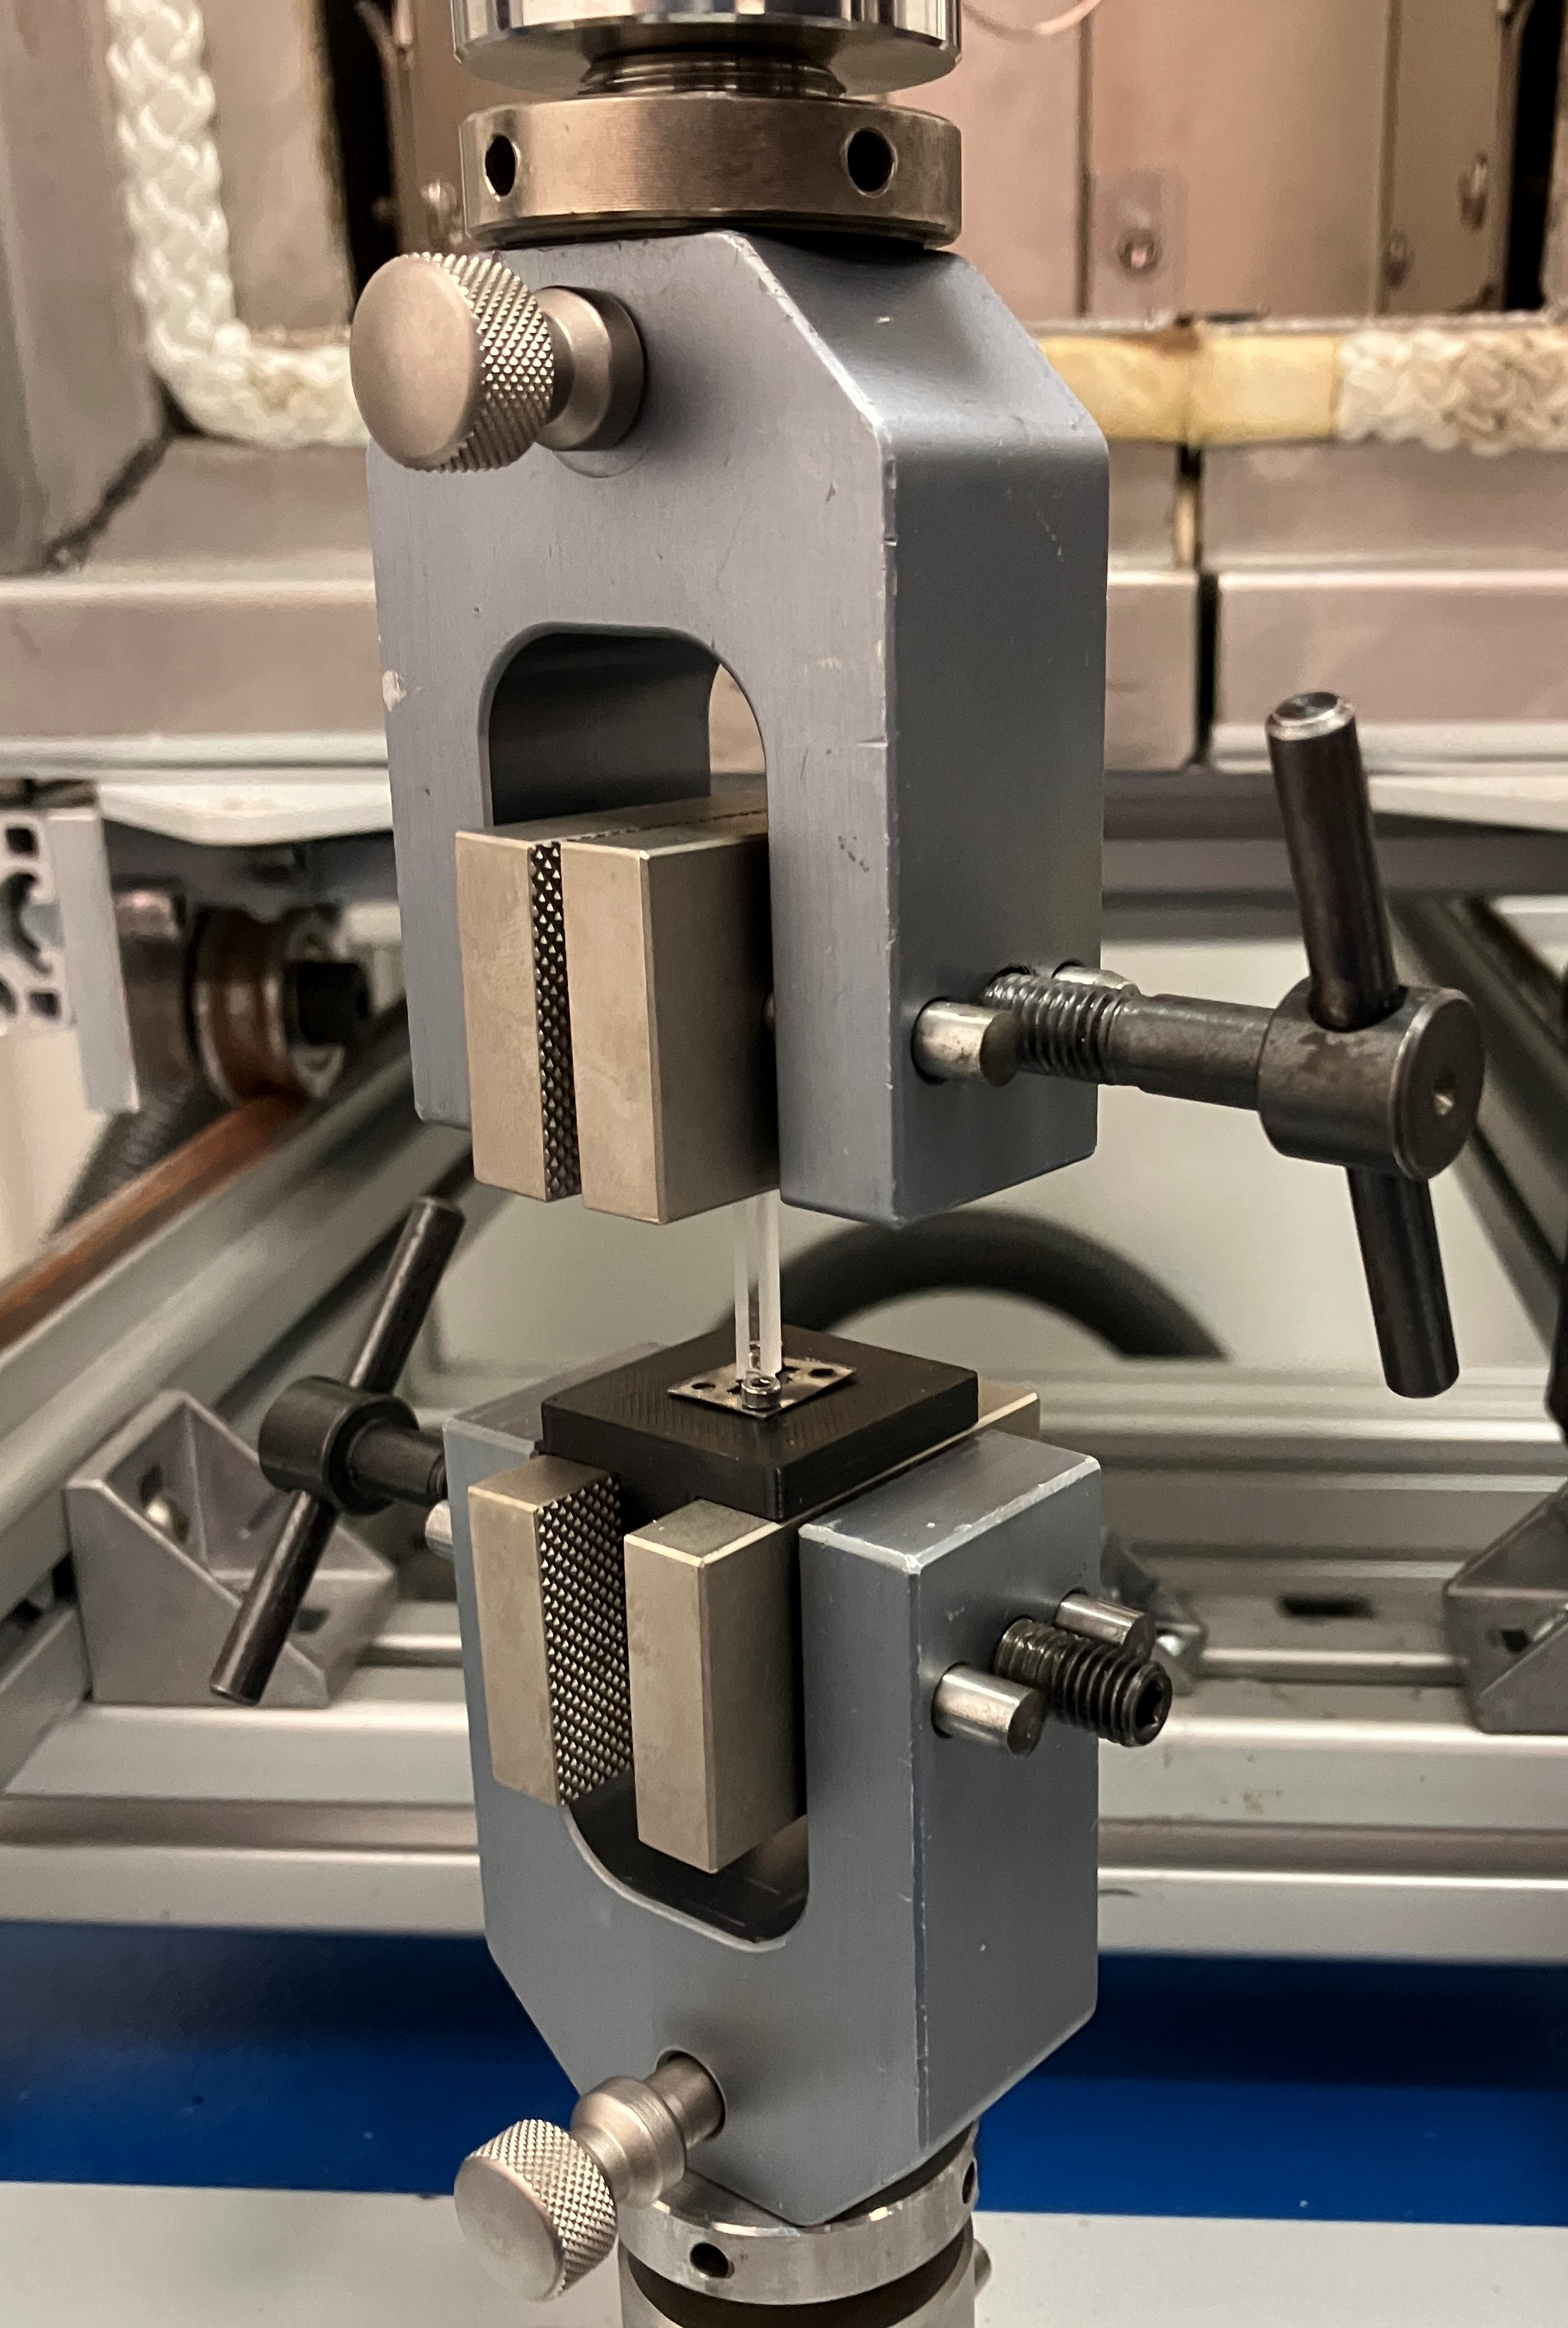
\includegraphics[width=6cm, height=9cm]{AufbauPullingMachineCloseup}
		\caption{}
	\end{subfigure}
	\caption{Setup on the Pulling Machine.}
	\label{fig:PullingMachineSetup}
\end{figure}

Because Glue dosaging varied a good amount, the Area is not assumed to be the bottom of the stamp. After Pulling, the glue is sticking on the stamp, outlining the area of the glue. The glue is analized under a microscope and the area is measured. With the Area and the maximum Force shortly before detaching, the Tensile stress is calculated. Then the experiment is repeated.



\subsection{detaching ice from PDMS}

1:2 and 4:1

